\documentclass[10pt,UTF8]{book} %% ctexart

\title{\textbf{矩阵微积分与自动微分}}
\author{钱锋\thanks{Email: strik0r.qf@gmail.com}${}^,$\thanks{
    西北工业大学软件学院, School of Software, Northwestern Polytechnical University, 西安 710072
}}

\usepackage{ctex}
\usepackage{graphicx}
\usepackage[toc]{multitoc}
\usepackage{booktabs}
\usepackage{longtable, diagbox}
\usepackage{amsthm, amssymb, amsmath, mathrsfs, mhchem}
\usepackage{tikz,circuitikz}
\usetikzlibrary{decorations.markings, angles, quotes}
\usetikzlibrary{shapes,arrows.meta,positioning}
\usepackage{tikz-cd}
\usepackage{pgfplots}
\usepackage{tikz-3dplot}
\usepackage{extpfeil}
\usepackage{diagbox}
\usepackage{float}
\usepackage{hyperref}
\hypersetup{hidelinks,
    colorlinks = true,
    allcolors = black,
    pdfstartview = Fit,
    breaklinks = true}
\usepackage{caption}
\usepackage{enumitem}
\usepackage{siunitx}
\usepackage{subcaption}
\usepackage{tasks}

\usepackage{fancyhdr} % 用于自定义页眉页脚


% 设置页眉页脚样式
\fancypagestyle{plain}{%
    \fancyhf{} % 清空页眉页脚
    \fancyhead[RO,LE]{·\thepage·} % 页眉显示页码, RO表示奇数页右侧, LE表示偶数页左侧
    \fancyhead[LO]{\nouppercase{\rightmark}} % 页眉显示小节标题, LO表示奇数页左侧
    \fancyhead[RE]{\nouppercase{\leftmark}} % 页眉显示章节标题, RE表示偶数页右侧
    \renewcommand{\headrulewidth}{0.4pt} % 设置页眉横线的宽度
    \renewcommand{\footrulewidth}{0pt} % 取消页脚横线
}

\renewcommand{\headrule}{\hrule width\textwidth height\headrulewidth\vskip-\headrulewidth}

% % 取消奇偶页的页眉偏移
% \fancyhfoffset[RO,LE]{0pt}

% % 取消奇偶页的页眉偏移
% \fancyhfoffset[RO,LE]{0pt}

% 定义取消页眉的命令
\newcommand{\cancelheader}{%
    \fancyhead{} % 清空页眉
    \renewcommand{\headrulewidth}{0pt} % 取消页眉横线
    \renewcommand{\footrulewidth}{0pt} % 设置页脚横线的宽度
}

\renewcommand{\chaptermark}[1]{\markboth{第 \thechapter 章 \hspace{1em} #1}{}} % 在章节标题前添加 "Chapter x: "
\renewcommand{\sectionmark}[1]{\markright{\thesection \, #1}} % 如果需要定义\rightmark,可以使用这行代码
\usepackage{titlesec} % 定义标题样式

% 设置 chapter 标题样式
\titleformat{\chapter}[hang]{\centering\heiti\Large\bfseries}{第\,\thechapter\,章}{1em}{}

% 定义 section 标题格式
\titleformat{\section}[hang]{\heiti\centering\large\bfseries}{\thesection}{1em}{}

% 定义 subsection 标题格式
\titleformat{\subsection}[hang]{\heiti\bfseries}{\textbf{\thesubsection}}{1em}{}

% 定义 subsubsection 标题格式
\setcounter{secnumdepth}{3}
\renewcommand\thesubsubsection{\arabic{subsubsection}.}
\titleformat{\subsubsection}[hang]{\kaishu}{\quad\quad\thesubsubsection\,\,}{0em}{}

% % 重新定义 textbf
% \let\oldtextbf\textbf
% \renewcommand{\textbf}[1]{{\heiti\oldtextbf{#1}}}

% % 在导言区重新定义 \normalsize 命令
% \makeatletter
% \renewcommand\normalsize{%
%    \@setfontsize\normalsize{10.5pt}{12pt}%
%    \abovedisplayskip 8\p@ \@plus2\p@ \@minus5\p@
%    \abovedisplayshortskip \z@ \@plus3\p@
%    \belowdisplayshortskip 6\p@ \@plus3\p@ \@minus3\p@
%    \belowdisplayskip \abovedisplayskip
%    \let\@listi\@listI}
% \makeatother



% 设置页边距和对齐
% \usepackage[
%     paperwidth=185mm,
%     paperheight=260mm,
%     top=35mm,
%     bottom=25mm,
%     left=18mm,
%     right=18mm,
%     footskip=15mm % 通过这里的值来调整页脚与正文内容的垂直距离
% ]{geometry}

\usepackage[
    paperwidth=210mm,
    paperheight=297mm,
    top=40mm,
    bottom=31.8mm,
    left=25.4mm,
    right=25.4mm,
    footskip=15mm % 通过这里的值来调整页脚与正文内容的垂直距离
]{geometry}

% \usepackage[
%     paperwidth=195mm,
%     paperheight=270mm,
%     top=40mm,
%     bottom=25mm,
%     left=23.5mm,
%     right=23.5mm,
%     footskip=15mm % 通过这里的值来调整页脚与正文内容的垂直距离
% ]{geometry}
\usepackage{mdframed}
\mdfsetup{
  linewidth=0.4pt,
  frametitlebackgroundcolor=white, % 或者 transparent
  frametitlefont=\heiti\bfseries,
  frametitleaboveskip=10pt,
  frametitlebelowskip=5pt,
  frametitlealignment=\raggedright % 新增此行
}
\usepackage{fontspec}
% 设置 Menlo 字体
\setmonofont{Menlo}
\usepackage{fancyvrb}
\usepackage{xcolor}
\usepackage{listings}

% \definecolor{string}{HTML}{067D17}
% \definecolor{comment}{HTML}{8C8C8C}
% \definecolor{keyword}{HTML}{0033B3}
% \definecolor{class_field}{HTML}{871094}

\lstset{breaklines}
%这条命令可以让LaTeX自动将长的代码行换行排版
\lstset{extendedchars=false}
%这一条命令可以解决代码跨页时,章节标题,页眉等汉字不显示的问题
\lstset{escapeinside={(*}{*)}}

\lstset{
    basicstyle=\small\ttfamily\heiti,
    numbers=left,
    numberstyle=\scriptsize\fontspec{Menlo}, % 使用 Menlo 字体
    stepnumber=1,
    numbersep=8pt,
    frame=leftline,
    xleftmargin=2em, % 调整代码块的左边界
    framexleftmargin=0pt, % 调整边框的位置
    breaklines=true,
    % postbreak=\mbox{\textcolor{red}{$\hookrightarrow$}\space},
    % keywordstyle=\bfseries\color{keyword},          % keyword style
    % commentstyle=\heiti\color{comment},       % comment style
    % stringstyle=\color[HTML]{067D17},
    showstringspaces=false,
    % string literal style
    % escapeinside={\%*}{*)},            % if you want to add LaTeX within your code
    % morekeywords={}               % if you want to add more keywords to the set
}

\usepackage{smartdiagram} % 表格对角线
\everymath{\displaystyle}
\usepackage{tasks}

\begin{document}
\newtheoremstyle{mytheoremstyle}
    {1.5ex}                                         % Space above
    {1.5ex}                                         % Space below
    {}                                              % Font for body
    {}                                              % Indent amount
    {\bfseries}                                     % Font for head
    {}                                              % Punctuation after head
    {0.5em plus 0.2em minus 0.1em}                  % Space after head
    {\thmname{#1}\thmnumber{ #2}.\thmnote{ (#3).}}

\theoremstyle{mytheoremstyle}
\newtheorem{definition}{定义}[section]
\newtheorem{example}{例}[section]
\newtheorem{exercise}{习题}[section]
\newtheorem{code}{程序清单}[section]
\newtheorem*{result}{运行结果}

\newtheoremstyle{my2theoremstyle}
    {1.5ex}                                         % Space above
    {1.5ex}                                         % Space below
    {\kaishu}                                              % Font for body
    {}                                              % Indent amount
    {\bfseries}                                     % Font for head
    {}                                              % Punctuation after head
    {0.5em plus 0.2em minus 0.1em}                  % Space after head
    {\thmname{#1}\thmnumber{ #2}.\thmnote{ (#3).}}

\theoremstyle{my2theoremstyle}
\newtheorem{thm}{定理}[section]
\newtheorem{law}{定律}[section]
\newtheorem{educt}{推论}
\newtheorem{prop}{命题}
\newtheorem{lemma}{引理}
\newtheorem{axiom}{公理}
\newtheorem{property}{性质}

\newtheoremstyle{my4theoremstyle}
    {1.5ex}                                         % Space above
    {1.5ex}                                         % Space below
    {}                                              % Font for body
    {}                                              % Indent amount
    {\bfseries}                                     % Font for head
    {}                                              % Punctuation after head
    {0.5em plus 0.2em minus 0.1em}                  % Space after head
    {\thmname{#1}.}

\theoremstyle{my4theoremstyle} \newtheorem*{sol}{解}

\newtheoremstyle{my3theoremstyle}
    {1.5ex}                                         % Space above
    {1.5ex}                                         % Space below
    {}                                              % Font for body
    {}                                              % Indent amount
    {\kaishu}                                       % Font for head
    {}                                              % Punctuation after head
    {0.5em plus 0.2em minus 0.1em}                  % Space after head
    {\thmname{#1}\thmnumber{ #2}.\thmnote{ (#3).}}

\theoremstyle{my3theoremstyle} \newtheorem*{remark}{注}
\newtheorem*{cmt}{评注}
% 使用 IEEE 样式
\ctikzset{logic ports=ieee}

\pagestyle{empty}
\begin{titlepage}
    \thispagestyle{empty}
    \centering
        \vspace*{3cm}
        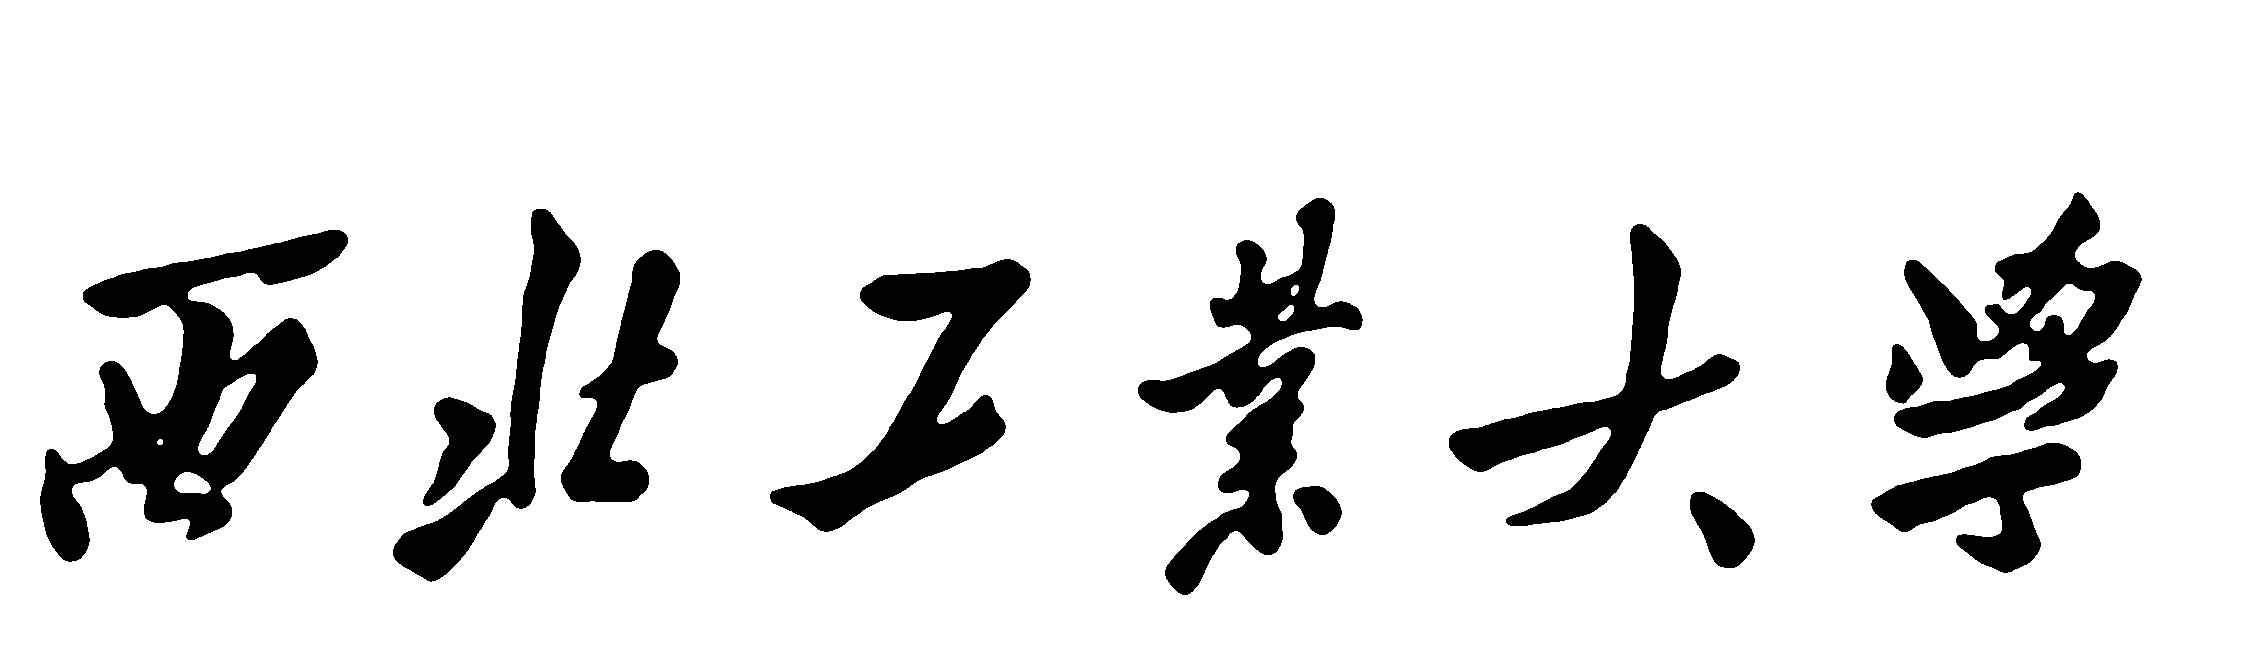
\includegraphics[width=0.5\textwidth]{pic/npu_2.png}\par
        \vspace{1em}
        
\includegraphics[width=0.5\textwidth]{pic/npu_1.png}\par
    \vspace*{1em}
        \begin{center}
            \Huge \heiti \textbf{矩阵微积分与自动微分}

            Matrix Calculus and Automatic Differentiation
        \end{center}

        \vspace{11em}
        \begin{center}
        \songti

        \kaishu 软件学院 \, \heiti\textbf{钱锋} \quad \songti 编
        \vspace{0.5em}

    \today
    \end{center}
\end{titlepage}
\cleardoublepage
\maketitle
\cleardoublepage
\frontmatter
\newpage
\pagestyle{plain}
\makeatother

\pagenumbering{roman} % 切换回罗马数字页码
\addtocontents{toc}{\protect\thispagestyle{empty}}
\pagestyle{plain}
{\tableofcontents}
\newpage
\thispagestyle{empty}
\cleardoublepage % 确保正文从奇数页开始


% 设置章节标题页的页眉和页脚为空白页样式
\makeatletter
\let\ps@plain\ps@empty
\makeatother

\mainmatter
\chapter{概述}

矩阵微积分主要讨论的是涉及向量、矩阵的函数的导数.

\section{定义与例子}

% \subsection{一阶导数的形式}

{\captionof{table}{一阶导数} % 表格标题
\label{一阶导数} % 交叉引用标签
\begin{longtable}{p{6em}p{8em}p{8em}p{8em}}
    \hline
    % 表头
    & \textbf{标量} $f$ & \textbf{向量} $\boldsymbol{f}$ & \textbf{矩阵} $\boldsymbol{F}$ \\
    \hline
    \endhead
    \hline
    \endfoot

    % 表格内容
    \textbf{标量} $x$ & 标量 $\partial f / \partial x$ 
    & 向量 $\partial \boldsymbol{f} / \partial x$ 
    & 矩阵 $\partial \boldsymbol{F} / \partial x$ \\ 
    \textbf{向量} $\boldsymbol{x}$ & 向量 $\partial f / \partial \boldsymbol{x}$
    
    \textbf{梯度} (gradiant) & Jacobi 矩阵
    
    $\partial \boldsymbol{f} / \partial \boldsymbol{x}$& 更高维的数组 \\ 
    \textbf{矩阵} $\boldsymbol{X}$ & 矩阵 $\partial \boldsymbol{f} / \partial \boldsymbol{X}$ & 更高维的数组 & 更高维的数组 \\
\end{longtable}}

表 \ref{一阶导数} 总结了不同形式输入和输出的函数的一阶导数的的形式, 其中,
每一行代表输入参数的一种可能性: 标量、向量或者矩阵, 而每一列则代表着返回值的一种
可能性.

本章中我们只研究表 \ref{一阶导数} 中提及的六种情况, 其中, 单变量标量值函数
$f(x)$ 的导数已经在微积分课程中讨论过了.

本章中的矩阵均采用分子布局.

\subsection{一元向量值函数的导数}

函数 $\boldsymbol{f}: x \mapsto [f_0(x), f_1(x), \cdots, f_{m-1}(x)]^\mathrm{T}$
接受一个标量输入 $x \in \mathbb{R}$, 并返回一个向量 $\boldsymbol{f}(x) \in \mathbb{R}^m$,
它的 $m$ 个分量分别为 $f_0(x), f_1(x), \cdots, f_{m-1}(x)$\footnote{
    为了方便在后期将我们的公式转换为代码, 我们的数组索引是从 $0$ 开始的.
}. 它的导数为
\[ \dfrac{\partial \boldsymbol{f}}{\partial x}
= \begin{bmatrix}
    \partial f_0 / \partial x \\ 
    \partial f_1 / \partial x \\ 
    \vdots \\ 
    \partial f_{m-1} / \partial x
\end{bmatrix}, \]
这就是说, {\kaishu 一元向量值函数的导数是一个向量, 它的每一个分量等于它对应的
分量函数对自变量的导数}. 我们在处理一元向量值函数的导数的时候, 只需要把 $\partial / \partial x$
放到向量符号当中就可以了.

\begin{example}
    设向量值函数 $\boldsymbol{f}(x) = \begin{bmatrix}
        2x^2 - 3x + 2 \\ 
        x^3 - 3
    \end{bmatrix}$,
    则 $\dfrac{\partial \boldsymbol{f}}{\partial x} = \begin{bmatrix}
        4x-3 \\ 
        3x^2
    \end{bmatrix}$.
\end{example}

\subsection{多元标量值函数的导数}

函数 $f: [x_0, x_1, \cdots, x_{m-1}] \mapsto f(\boldsymbol{x})$
接受一个矢量输入 $\boldsymbol{x} \in \mathbb{R}^m$, 并返回一个标量值
$f(\boldsymbol{x}) \in \mathbb{R}$. 它的导数为
\[ \dfrac{\partial f}{\partial \boldsymbol{x}}
= \begin{bmatrix}
    \dfrac{\partial f}{\partial x_0 },
    \dfrac{\partial f}{\partial x_1},
    \cdots,
    \dfrac{\partial f}{\partial x_{m-1}}
\end{bmatrix}, \]
为了在我们的公式中采用分子布局, 我们将 $\partial f/\partial \boldsymbol{x}$
转置以使其成为一个列向量, 并将其定义为多元标量值函数的\textbf{梯度} (gradient),
用 Hamilton 算子 $\nabla$ 表示, 即
\[ \nabla f(\boldsymbol{x}) = \begin{bmatrix}
    \dfrac{\partial f}{\partial x_0 } \\[\bigskipamount]
    \dfrac{\partial f}{\partial x_1} \\[\bigskipamount]
    \vdots \\[\bigskipamount]
    \dfrac{\partial f}{\partial x_{m-1}}
\end{bmatrix} \]

\setcounter{property}{0}
\begin{property}[齐次性]
    $\dfrac{\partial }{\partial \boldsymbol{x}}(af)
    =a \dfrac{\partial f}{\partial \boldsymbol{x}}$.
    \begin{proof}
        $\dfrac{\partial }{\partial \boldsymbol{x}}(af)
        = \begin{bmatrix}
            \dfrac{\partial (af)}{\partial x_0},
            \dfrac{\partial (af)}{\partial x_1},
            \cdots,
            \dfrac{\partial (af)}{\partial x_{m-1}}
        \end{bmatrix}
        =a \dfrac{\partial f}{\partial \boldsymbol{x}}$.
    \end{proof}
\end{property}
\begin{property}[叠加性]
    $\dfrac{\partial}{\partial \boldsymbol{x}}(f+g)
    = \dfrac{\partial f}{\partial \boldsymbol{x}}
    + \dfrac{\partial g}{\partial \boldsymbol{x}}$.
    \begin{proof}
        由定义可知, 
        \[ 
        \begin{aligned}
            \dfrac{\partial}{\partial \boldsymbol{x}}(f+g)
            & = \begin{bmatrix}
                \dfrac{\partial (f+g)}{\partial x_0},
                \dfrac{\partial (f+g)}{\partial x_1},
                \cdots,
                \dfrac{\partial (f+g)}{\partial x_{m-1}}
            \end{bmatrix} \\
            & = \begin{bmatrix}
                \dfrac{\partial f}{\partial x_0}+ \dfrac{\partial g}{\partial x_0},
                \dfrac{\partial f}{\partial x_1}+\dfrac{\partial g}{\partial x_1},
                \cdots,
                \dfrac{\partial f}{\partial x_{m-1}}+\dfrac{\partial g}{\partial x_{m-1}}
            \end{bmatrix},
        \end{aligned} \]
        根据一元函数的导数的可加性可知结论成立.
    \end{proof}
\end{property}
\begin{property}[乘积法则]
    $\dfrac{\partial}{\partial \boldsymbol{x}}(fg)
    = f\dfrac{\partial g}{\partial \boldsymbol{x}} 
    + g\dfrac{\partial x}{\partial \boldsymbol{x}}$.
    \begin{proof}
        这可以由一元函数的乘积法则直接导出.
    \end{proof}
\end{property}
\begin{property}[链式法则]
    如果 $f: \mathbb{R} \to \mathbb{R}$, $g: \mathbb{R}^m \to \mathbb{R}$.
    则 $\dfrac{\partial}{\partial \boldsymbol{x}}f(g(\boldsymbol{x}))
    = \dfrac{\partial f}{\partial g}
    \dfrac{\partial g}{\partial \boldsymbol{x}}$.
\end{property}

\subsection{多元向量值函数的导数}

函数 $\boldsymbol{f}: [x_0, x_1, \cdots, x_{m-1}]^\mathrm{T} \mapsto 
[\boldsymbol{f}_0(x_0), \boldsymbol{f}_1(x_1), \cdots, \boldsymbol{f}_{n-1}(x_{m-1})]^\mathrm{T}$
接受一个向量 $\boldsymbol{x} \in \mathbb{R}^m$ 作为输入, 并返回一个向量
$\boldsymbol{f}(\boldsymbol{x}) \in \mathbb{R}^n$ 作为输出.
事实上, 我们可以把 $\boldsymbol{f}$ 分解成若干个多元标量值函数,
即
\[ \boldsymbol{f}(\boldsymbol{x})
= \begin{bmatrix}
    f_0(\boldsymbol{x}) \\
    f_1(\boldsymbol{x}) \\
    \vdots \\ 
    f_{n-1}(\boldsymbol{x}) \\
\end{bmatrix}, \]
为了求解它关于 $\boldsymbol{x}$ 的导数, 我们把 $\partial / \partial \boldsymbol{x}$
放进向量符号中,
\[ \dfrac{\partial \boldsymbol{f}}{\partial \boldsymbol{x}}
= \begin{bmatrix}
    \partial f_0 / \partial \boldsymbol{x} \\
    \partial f_1 / \partial \boldsymbol{x}\\
    \vdots \\ 
    \partial f_{n-1} / \partial \boldsymbol{x} \\
\end{bmatrix} \]
而这时 $\partial f_i / \partial \boldsymbol{x}$ 就是多元标量值函数的导数,
因此
\[ \dfrac{\partial \boldsymbol{f}}{\partial \boldsymbol{x}}
= \begin{bmatrix}
    \dfrac{\partial f_0}{\partial x_0} & \dfrac{\partial f_0}{\partial x_1} & \cdots & \dfrac{\partial f_0}{\partial x_{m-1}} \\[\bigskipamount]
    \dfrac{\partial f_1}{\partial x_0} & \dfrac{\partial f_1}{\partial x_1} & \cdots & \dfrac{\partial f_1}{\partial x_{m-1}} \\[\bigskipamount]
    \vdots & \vdots & \ddots & \vdots \\[\bigskipamount]
    \dfrac{\partial f_{n-1}}{\partial x_0} & \dfrac{\partial f_{n-1}}{\partial x_1} & \cdots & \dfrac{\partial f_{n-1}}{\partial x_{m-1}}
\end{bmatrix}, \]
它的每一行都是 $\left(\nabla f_i(\boldsymbol{x})\right)^\mathrm{T}$.

\subsection{一元矩阵值函数的导数}

函数 $\boldsymbol{F}: \mathbb{R} \to \mathbb{R}^{n \times m}$
接受一个标量输入, 返回一个矩阵
\[ \boldsymbol{F} = \begin{bmatrix}
    f_{00}(x) & f_{01}(x) & \cdots & f_{1,m-1}(x) \\
    f_{10}(x) & f_{11}(x) & \cdots & f_{1,m-1}(x) \\
    \vdots & \vdots & \ddots & \vdots \\
    f_{n-1,0}(x) & f_{n-1,1}(x) & \cdots & f_{n-1,m-1}(x)
\end{bmatrix}, \]
它的导数为
\[ \dfrac{\partial \boldsymbol{F}}{\partial x}
=  \begin{bmatrix}
    \dfrac{\partial f_{00}}{\partial x} & \dfrac{\partial f_{01}}{\partial x} & \cdots & \dfrac{\partial f_{0, m-1}}{\partial x} \\[\bigskipamount]
    \dfrac{\partial f_{10}}{\partial x} & \dfrac{\partial f_{11}}{\partial x} & \cdots & \dfrac{\partial f_{1, m-1}}{\partial x} \\[\bigskipamount]
    \vdots & \vdots & \ddots & \vdots \\[\bigskipamount]
    \dfrac{\partial f_{n-1,0}}{\partial x} & \dfrac{\partial f_{n-1,1}}{\partial x} & \cdots & \dfrac{\partial f_{n-1, m-1}}{\partial x}
\end{bmatrix}.\]

\subsection{标量值矩阵函数的导数}

函数 $f: \mathbb{R}^{n \times m} \to \mathbb{R}$
接受一个矩阵 $\boldsymbol{X}$ 作为输入, 并返回一个标量值.
它的导数为
\[ \dfrac{\partial f}{\partial \boldsymbol{X}} = 
\begin{bmatrix}
    \dfrac{\partial f}{\partial x_{00}} & \dfrac{\partial f}{\partial x_{10}} & \cdots & \dfrac{\partial f}{\partial x_{n-1,0}} \\[\bigskipamount]
    \dfrac{\partial f}{\partial x_{01}} & \dfrac{\partial f}{\partial x_{11}} & \cdots & \dfrac{\partial f}{\partial x_{n-1,1}} \\[\bigskipamount]
    \vdots & \vdots & \ddots & \vdots \\[\bigskipamount]
    \dfrac{\partial f}{\partial x_{0,m-1}} & \dfrac{\partial f}{\partial x_{1,m-1}} & \cdots & \dfrac{\partial f}{\partial x_{n-1,m-1}}
\end{bmatrix}. \]

% \subsection{自动微分}

% 典型的微分运算往往是符号运算 (symbolic calculus), 
% 在 MATLAB 或者 Mathematica 这样的科学计算软件中.
% 对于少部分函数的导数, 我们也可以采用数值微分 (numerical differentiation)
% 来解决, 例如, 我们可以通过计算一个极小的有限扰动 $h$ 下
% $f(x+h) - f(x)$ 与 $h$ 的比值来得到导数的值.

% 自动微分 (automatic differentiation) 不同于符号微分, 也不同于数值微分,
% 它涉及到了计算机科学中的更多的复杂的技术. 如今, 自动微分已经被广泛的应用于机器学习
% 中, 了解自动微分的一些底层原理, 有助于我们更好的使用这些工具 (而不是单纯的调用
% 深度学习框架或其他各种库, 或者自动微分软件所提供的 API).

% \subsection{单变量标量值函数}

% 单变量函数 (single variable funtion) 又称为\textbf{标量函数}
% (function of scalars), 这是因为它的自变量是标量. 函数值为标量的函数
% 称为\textbf{标量值函数} (scalar function), 请不要被这些类似的名词
% 所迷惑, 一定要体会到这个名词中 “值” 这个字的含金量. 总之,
% 处理标量值标量函数 (就是输出标量的单变量函数) 的微分总是简单的:
% \begin{itemize}[itemsep=0pt]
%     \item 单变量函数的导数仍为单变量函数;
%     \item 如果函数的增量可以写成
%     \[ f(x)-f(x_0) \approx f'(x_0) (x - x_0) \]
%     的形式, 那么我们称 $f$ 是\textbf{可微的} (differentiable),
%     $f'(x_0) (x - x_0)$ 称为函数 $f$ 的线性化 (linearization).
%     事实上, 可微函数具有局部线性性, 即 {\kaishu 可微函数在某点处的变化量
%     大体上与该点所在区域的宽度线性相关}.
%     我们也用符号 $\Delta$ 来表示有限的扰动 (finite perturbation),
%     因此上式也可以写为
%     \[ \Delta f \approx f'(x_0)\Delta x. \]
% \end{itemize}

% 在上面的两个式子中, $\approx$ 实际上表示了近似值与真实值之间的差距是扰动
% $\Delta x$ 的高阶无穷小, 在微积分中, 我们通常也采用
% \[ \mathrm{d}f = f'(x_0)\mathrm{d}x \]
% 来表示函数的可微性, 注意在这一个式子中, 我们直接使用等号, 而不是约等号.
% 这就是说, $\mathrm{d}f$ 是 $f$ 的增量中的线性部分, 我们通常称其为
% 增量的\textbf{线性主部} (linear main part).
% 如果我们把函数增量的线性主部 $\mathrm{d}f$ 显式地表示为
% $f(x_0 + \mathrm{d}x) - f(x_0)$, 那么我们有
% \[ f(x_0 + \mathrm{d} x) = f(x_0) + f'(x_0) \mathrm{d}x. \]



% \begin{example}
%     $\mathrm{d}(x^3) = 3x^2 \mathrm{d}x$, 导数为标量 $3x^2$,
%     你可以理解为我们对无穷小标量 $\mathrm{d}x$ 与标量 $3x^2$ 做了标量乘法
%     运算.
% \end{example}
% \begin{example}
%     $\mathrm{d}\left(\boldsymbol{x}^\mathrm{T}\boldsymbol{x}\right)
%     =2\boldsymbol{x}^\mathrm{T} \mathrm{d}\boldsymbol{x}$,
%     它的导数是一个矢量 $2\boldsymbol{x}^\mathrm{T}$, 这个结果实际上是矢量 $2\boldsymbol{x}$ 与无穷小矢量 
%     $\mathrm{d}\boldsymbol{x}$ 的点乘积.
% \end{example}
% \begin{example}
%     $\mathrm{d}\left( \boldsymbol{X}^2 \right) = \boldsymbol{X}
%     \mathrm{d}\boldsymbol{X} + \mathrm{d}\boldsymbol{X}\, \boldsymbol{X}$.
%     它的结果是用 $\boldsymbol{X}$ 分别左乘、右乘无穷小矩阵 $\mathrm{d}\boldsymbol{X}$
%     再相加, 是一个矩阵.
% \end{example}

% \subsection{矩阵微分的乘积法则}

% \[ \mathrm{d}\left(\boldsymbol{AB}\right)
% = \left(\mathrm{d}\boldsymbol{A}\right)\boldsymbol{B}
% + \boldsymbol{A}\left(\mathrm{d}\boldsymbol{B}\right). \]

\appendix
% 设置 chapter 标题样式
\titleformat{\chapter}[hang]{\centering\heiti\Large\bfseries}{附录\,\thechapter}{1em}{}
\renewcommand{\chaptermark}[1]{\markboth{附录 \thechapter\, #1}{}} % 在章节标题前添加 "Chapter x: "

\onecolumn
\begin{thebibliography}{1}
    \addcontentsline{toc}{chapter}{参考文献}

\end{thebibliography}

\newpage
\thispagestyle{empty}
\vspace*{5cm}
\begin{center}
    \includegraphics*[width=\textwidth]{pic/i_love_npu.jpeg}
    \large
    公诚勇毅 \quad 永矢毋忘

    中华灿烂 \quad 工大无疆
\end{center}
\vspace*{13em}
\begin{center}
    \small
    本文档由\textbf{钱锋}编写, 钱锋保留一切权利.

    文档中出现的部分素材来源于网络, 笔者承诺这些素材仅供学习交流之用, 
    它们的原作者保留一切权利.

    2023 年 \quad 西北工业大学 \quad 中国西安 
\end{center}

\end{document}